\subsection{Сегментация изображений при помощи разрезов на графах}
Сегментация изображений является одним из важных шагов в процессе компьютерного зрения. Сегментация изображений играет большую роль в анализе изображений и в получении важной информации из изображений.

На практике сегментация изображений имеет две сложные проблемы: слабые границы и структуры. Первая проблема состоит в нахождении слабых границ, когда они являются частью соответствующей границы. Вторая проблемма заключается в разделении сложных структур в изображении \cite{Sagiv2006, Raviv2007}. На самом деле, такие ситуации часто возникают в практике. В этом случае сегментация становится неясной без добавления априорной информации пользователей. Поэтому, использование методов сегментации изображений с учителем широко используется.

В настоящее время существует много алгоритмов предлагаемых для решения задач сегментации изображений. Существует три типа алгоритмов сегментации обучения с учителем, основанных на исходной информации от пользователей:

\begin{itemize}
	\item Первый тип является результатом сегментации на основании желательных границ, например Intelligent Scissors \cite{Mortensen1995};
	\item Второй тип является  результатом сегментации на основании исходных границ, которые находятся близко с желательными границами, например Active Contour \cite{Lankton} и Set Level \cite{Lie2006};
	\item Третий тип является результатом сегментации на основании маркировки пикселей, которые задаются пользователами.
\end{itemize}
Одним из популярных подходов является метод разреза на графах, которые основаны на функции энергии. В этом методе изображение представляется как взвешенный неориентированный граф. Обычно пиксель или группа пикселей ассоциируется вершиной, а веса рёбер определяют (не)похожесть соседних пикселей. Затем граф (изображение) разрезается согласно критерию, созданному для получения «хороших» кластеров. Каждая часть вершин (пикселей), получаемая этими алгоритмами, считается объектом на изображении.

\textbf{Проблема о максимальном потоке} (maximum flow problem): найти поток $f$ такой, что величина потока максимальна. 
\[
f: \sum_u f\left(u\rightarrow v\right)=\sum_wf\left(v\rightarrow w\right). 
\]

Величина потока (value of flow) — сумма потоков из источника.
\[
\left|f\right|:= \sum_w f \left(s\rightarrow w\right) - \sum_u f\left(u\rightarrow s\right).
\]

\textbf{Минимальный разрез} — разрез с минимальной пропускной способностью. 
$C_{min} \left(A,B\right)=\sum_{u\in S, v \in T} W_{uv}$.

Разрез (s-t cut) — разбиение множества всех вершин V на два подмножества $A$ и $B$ таких, что $s\in A $, $t\in B$, причем пересечение $A$ и $B$ равно пустому множеству. Если рассматривать весовые коэффициенты, связанные с каждым узлом в качестве емкости потока, можно показать, что максимальное количество энергии потока от источника равно емкости минимального разреза. Поэтому проблема минимального разреза также известна как проблема максимального потока. Нужно выбрать необходимый поток и необходимый разрез $\left(S, T\right)$, а затем следить неравенством \cite{Boykov12001}:
\begin{equation}\label{eq21}
\left|f\right| = \sum_w f\left(s\rightarrow w\right) - \sum_u f \left(u\rightarrow s\right),
\end{equation}
\[
=\sum_{v\in S}\left(\sum_w f \left(v \rightarrow w \right) - \sum_u f\left( u \rightarrow v \right) \right),
\]
\[
= \sum_{v \in S} \left(\sum_{w \in T} f \left( v \rightarrow w\right) - \sum_{u \in T} f \left( u \rightarrow v \right)\right),
\]
\[
\leq \sum_{v \in S}\sum_{w \in T} f \left( v \rightarrow w \right) после  f \left(u \rightarrow v\right) \geq 0,
\]
\[
\leq \sum_{v \in S}\sum_{w \in T} c \left(v\rightarrow w \right)  после f \left(u \rightarrow v \right) \leq c \left( v \rightarrow w\right),
\]
\[
=\left\|S, T\right\|.
\]

Грань между пиксельной $i$ и $j$ будем обозначать $W^I_{ij}$ и терминал весов между пиксельной $i$ и источником $\left(s\right)$ и мойкой $\left(t\right)$. $W^s_i$ и $W^t_i$ соответственно задаются \cite{Parvathy}:
\begin{equation}\label{eq22}
W^i_{ij} = e^{\left(-\frac{r\left(i,j\right)}{\sigma R}\right)}e^{\left(-\frac{\left\|w\left(i\right)-w\left(j\right)\right\|^2}{\sigma W}\right)},
\end{equation}
\begin{equation}\label{eq23}
W^s_i = \frac{p\left(w\left(i\right)| i \in s\right)}{p \left(w \left(i\right)\right)|i \in s + p \left(w\left(i\right)|i \in t\right)},
\end{equation}
\begin{equation}\label{eq24}
W^t_i = \frac{p\left(w\left(i\right) | i \in t\right)}{p \left(w \left(i\right)\right)|i \in s + p \left(w\left(i\right)|i \in t\right)}.
\end{equation}
Где:

\begin{itemize}
	\item $r\left(i,j\right)$ расстояние между пиксельной $i$ и $j$;
	\item $\left\|.\right\|$ обозначает евклидову норму;
	\item $\sigma R$ и $\sigma W$ настраивают параметры, взвешивая различные значения;
	\item $W^I_{ij}$ содержит сходство между пикселями;
	\item $W^s_i$, $W^t_i$ описывает пиксель фона и переднего плана соответственно.
\end{itemize}
В сегментации изображений обычно имеется задача разбиения на $2$ области : объект foreground и фон. Данный метод стал основой большинства современных наилучших методов интерактивной сегментации, так что остановимся на этом алгоритме подробнее.

На входе данный алгоритм разреза графов получает исходные данные изображений и добавление информаций от пользователей: количество пикселей объекта, области вокруг объекта, приблизительную границу объекта \cite{Boykov2001}. Чтобы ограничить ошибки в сегментации изображения для решения требований практических задачи, пользователь обеспечит необходимые данные каждому случаю. Дан граф $G\left(V,E\right)$ с пропускной способностью $c\left(u,v\right)$ и потоком $f\left(u,v\right)=0$ для ребер из $u$ в $v$. Необходимо найти максимальный поток (Max – flow) из источника $s$  (source) в сток $t$ (sink). На каждом шаге алгоритма действуют те же условия, что и для всех потоков \cite{Cormen2001}:

\begin{itemize}
	\item $f\left(u,v\right) \leq c\left(u,v\right)$ - Это поток из u в v не превосходит пропускной способности;
	\item $f\left(u,v\right) =-f\left(v,u\right)$;
	\item $\sum_vf\left(u,v\right)=0 \leftrightarrow f_{in}\left(u\right) =f_{out}\left(v\right)$ для всех узлов $u$, кроме $s$ и $t$;
	\item Остаточная сеть $G_f\left(V,E_f\right)$ - сеть с  пропускной способностью $c_f\left(u,v\right)=c\left(u,v\right)-f\left(u,v\right)$ и без потока Ford – Fulkerson (1956) \cite{Ford1956}. Максимальный поток на основе алгоритма (\ref{img12}).
\end{itemize}

\begin{figure}[ht!]
\centering
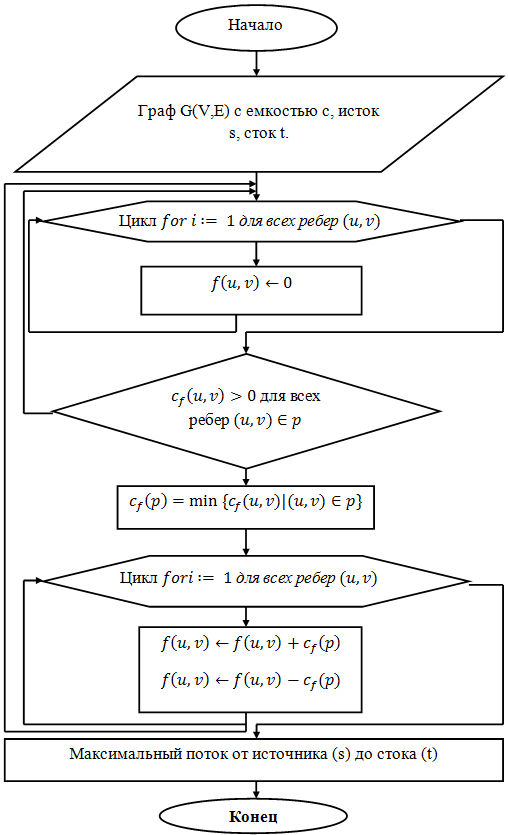
\includegraphics [scale=1] {images/h12.png}
\begin{center}
%\captionsetup{justification=justified, labelsep=period}
\caption{Блок-схема алгоритма разреза на графах.} \label{img12}
\end{center}
\end{figure}

Метод разреза графов находит сильные локальные минимумы энергетической функции. Метод достаточно мощный, чтобы решать множество полезных задач, и он может быть применен к решению проблемы графика min-среза. 
\begin{equation}\label{eq25}
E\left(f\right) = \sum_{p \in P}D_p\left(f_p\right)+\sum_{p,q \in N}V_{p,q}\left(f_p,f_q\right).
\end{equation}
Найти маркировки $f:P\rightarrow L$ , что сводит к минимуму $E\left(f\right)$ из множеств пикселей $P$, набор этикеток $L,N \in P$ является система соседства по пикселям. $D_p\left(f_p\right)$ является функцией, которая получена из данных наблюдений, и которая измеряет стоимость присвоения метки $f_p$ на пиксель $p$. $V_{\left(p,q\right)} \left(f_p,f_q\right)$ , и измеряет стоимость присвоения метки $f_p$,$f_q$ на соседние пиксели $p$, $q$. Используется для улучшения пространственного сглаживания \cite{Boykovv2001, Boykov2004}.

На каждом шаге алгоритм выполняет каждый поток, который соединяет от $s$ к $t$. Сложность алгоритма зависит от числа ребер, осуществляется по индукции всех потоков. Движение потока увеличивается, по меньшей мере один раз на каждом шаге алгоритма. Поэтому, сложность алгоритма не превосходит $O\left(f\right)$, где  $f$ - максимальный поток в графе.  $E$ - это число ребер графа, так что сложность будет $О\left(E\ast f\right)$.

После этого в полученном графе находится минимальный разрез, который делит граф на $2$ части. Вес ребер между метками обеспечивает выполнение заданных пользователем ограничений: маркировки объекта будут отнесены к объекту, маркировки фона - к фону.
